\documentclass[10pt]{IEEEtran}
\pdfoutput=1

\usepackage{graphicx}
\usepackage{hyperref}
\usepackage[utf8]{inputenc}
\usepackage{listings}
\usepackage[table]{xcolor}
\usepackage{pdfpages}
\usepackage{algpseudocode}
\usepackage{natbib}
\usepackage{tikz}
\usetikzlibrary{shapes,shadows,arrows}

%style to be used on block diagrams
\tikzstyle{block} = [draw,rectangle, fill=white]
\tikzstyle{line} = [draw,thick]
\tikzstyle{arrowLine} = [draw,-stealth,thick]

%style to be used on flow charts diagrams
\tikzstyle{startstop} = [rectangle, rounded corners, minimum width=2.5cm,
minimum height=0.75cm,text centered, draw=black,fill=red!30]
\tikzstyle{io} = [trapezium, trapezium left angle=70,trapezium right angle=110,
minimum width=2.5cm,minimum height=0.75cm,text centered, draw=black,fill=blue!30]
\tikzstyle{process} = [rectangle, minimum width=2.25cm, minimum height=0.75cm, text centered, draw=black, fill=orange!30]
\tikzstyle{decision} = [diamond, minimum width=2cm, minimum height=0.5cm, 
text centered, draw=black,fill=green!30]
\tikzstyle{flowArrow} = [thick,->,->=stealth]


\hypersetup{colorlinks=true,citecolor=[rgb]{0,0.0,0}}


\title{Data mining with python: \\Automated FOREX trading}
\author{
	Kevin Voss Sjøbeck(s103451)\\
	\and
	Benjamin Maksuti(s103449)\\
	\and
	Anders Wessberg(s103477)
}


\begin{document}
\maketitle

\begin{abstract}
This project will utilize the oandapy API to get realtime data from the currency market to analyse, as well as enter and exit trades on based on the analytics. In the analytics we are going to use a short and a long moving averages, furthermore we are going to use MCAD as an extra precaution before we enter trades and use recovery zones to prevent losses on the account
\end{abstract}

\section{Introduction}
Here will be written an introduction


\section{Analysis}

\subsection{Getting data}
We obtain all the financial data of the financial instrument EUR vs USD, on a 5 minute timeframe from oanda, using their own REST API for python. From oanda's API we get the financial charts of a 7 year time period, going from 2007-10-01 to 2014-10-20. After obtaining the data, it is stored in json fileformat in a file called "fxdata.txt", this data will then be used both to form our hypothosis of forex trading on the EUR vs USD currency pair, as well as performing a trading simulation on this set of data. However in order for us to use the naive Bayes classifier, we need to have two dataset's and not just a single one. In our domain the one dataset needs to be the trades which gained profit, and the other set needs consist of the trades which lost. We then have the possibility to analyze the data with different sets of features.\\
\\
The pseudo code of the random trading algorithm, where we will keep the orders for no more than 20 minutes:

\begin{center}
\begin{algorithmic}
\While{$streamFinancialData$}
	\State {$i = random(0,10)$}
	\If {$i = 0$}
    	\State {$openOrder(short)$}
	\ElsIf{$i = 1$}
    	\State $openOrder(long)$	    
	\EndIf
	\For{$order\: in\: orders$}	
		\If{$order.hasProfit()$}
			\State{$profitList.append(order)$}
			\State{$order.close()$}
		\ElsIf{$order.hasLoss()$}
			\State{$lossList.append(order)$}
			\State{$order.close()$}
		\ElsIf{$order.duration >= 4$}
			\State{$order.close()$}
		\Else
			\State{$order.duration += 1$}
		\EndIf
	\EndFor
\EndWhile
\State{$saveListToFile(profitList,"profit.txt")$}
\State{$saveListToFile(lossList,"loss.txt")$}
\end{algorithmic}
\end{center}

This algorithm should theoretically give us equally profitable trades in both the long and the short direction.

\subsection{Specific features}
To analyse the data we use a supervised classification learning algorithm, or to be more specific we use a naive Bayes classifier, the idea is to use a naive Bayes classifier on our financial data we gathered using our random algorithm. This isn't a new concept, in fact there are a couple of scientific articles on this already, as can be seen in the article by KAWABATA and TAKATA \cite{fxNaiveBayes}. We will train the classifier on some specific features, however we will only use 2-3 features per training round. The training will be made in two rounds and the features are the following
\begin{itemize}
	\item{CrossGraph(SMA(10,40))}
	\item{RSI(period=100)}
	\item{openBid(period=1)}
	\item{closeBid(period=1)}
	\item{volume(period=1)}
	\item{spread(period=1)}
	%\item{Parabolic SAR default settings (0.02, 0.2)}
	%\item{MACD default settings (fast=12, slow = 15, period=9)}
\end{itemize}

The first round of features, is using some of the most common technical indicators on the FX market, this should give a good indication if those are just famous for being simple or if you actually are able to earn profit using these indicators. The second round another of the more simple techniques that some of the professional FX traders should use according to chat on the different trading forums, this isn't really a technical indicator, it is much more a way to look at the market and only make a trade if the current price reaches a specific value. Our hypothosis is that the traders who use price actions looks only at the price, so that is exactly what we are going to do as well, and by giving the classifier the features of openBid, closeBid, volume, and spread we hope to achive the behaviour of a price action trader. On the third and last round of features, we searched the internet for a forex trading strategy on the EUR vs USD pair, to see how our strategies of the first two rounds of features compare to a random strategy you can find on the internet. The strategy we found consist of using SAR indicator as well as three different MACD indicators.

\begin{figure}
\begin{center}
	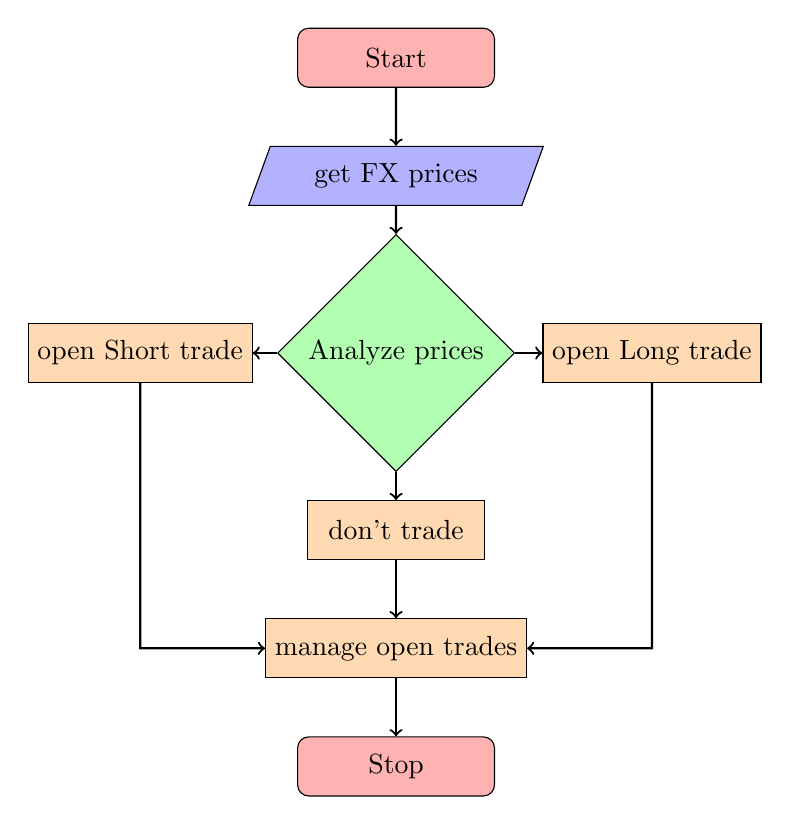
\begin{tikzpicture}[node distance=2cm]
		%blocks
		\node[startstop](start){Start};
		\node[io, below of=start,yshift=0.5cm](fx_price){get FX prices};
		\node[decision, below of=fx_price,yshift=-0.25cm](analyze){Analyze prices};	
		\node[process, right of=analyze, xshift=1.25cm](long){open Long trade};
		\node[process, left of=analyze, xshift=-1.25cm](short){open Short trade};
		\node[process, below of=analyze,yshift=-0.25cm](no_trade){don't trade};		
		\node[process, below of=no_trade,yshift=0.5cm](manage){manage open trades};				
		\node[startstop, below of=manage,yshift=0.5cm](stop){Stop};		
		
		%arrows			
		\draw[flowArrow](start)--(fx_price);
		\draw[flowArrow](fx_price)--(analyze);		
		\draw[flowArrow](analyze)--(long);		
		\draw[flowArrow](analyze)--(short);						
		\draw[flowArrow](analyze)--(no_trade);						
		\draw[flowArrow](no_trade)--(manage);
		\draw[flowArrow](short)--(-3.25,-7.5)--(manage);		
		\draw[flowArrow](long)--(3.25,-7.5)--(manage);		
		\draw[flowArrow](manage)--(stop);		
	\end{tikzpicture}
\end{center}
\caption{Flowchart of decision making}
\end{figure}


\section{Design}
Before we start trading, we need to train our classifier based on the feature set we mentioned in the analysis. After the training is completed, we can then start trading based on our historical data. 
After a completed run of the historical data, the result of the trade is then shown on a graph, showing the profit/loss of a 5 minute interval. Figure 1. is showing a flowchart of how the trading cycles. From this we know that we need a driver to run the program, that retrieves signals from either the Random trader or the classifier, depending on what is chosen. The driver then creates orders of trades, but to keep track of them all, we need an order manager. The driver also needs to be able to withdraw/deposit money to an account manager. Figure 2. is showing the class diagram on how we will implement it all.\\



\begin{figure}
\begin{center}
	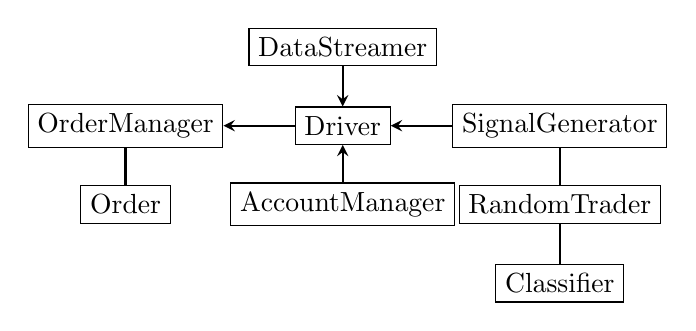
\begin{tikzpicture}
		\node[block](streamer){DataStreamer};
		\node[block,below of=streamer](driver){Driver};		
		\node[block,below of=driver](accountManager){AccountManager};				
		\node[block,left of=driver,xshift=-5em](orderManager){OrderManager};
		\node[block,below of=orderManager](order){Order};		
		\node[block,right of=driver,xshift=5em](signalGenerator){SignalGenerator};
		\node[block,below of=signalGenerator](random){RandomTrader};				
		\node[block,below of=random](Classifier){Classifier};						
		%arrows
		\path[arrowLine](streamer)--(driver);		
		\path[arrowLine](accountManager)--(driver);				
		\path[arrowLine](driver)--(orderManager);
		\path[line](orderManager)--(order);
		\path[arrowLine](signalGenerator)--(driver);
		\path[line](signalGenerator)--(random);				
		\path[line](random)--(Classifier);						
	\end{tikzpicture}
\end{center}
\caption{Overview of Classes}
\end{figure}




\section{Implementation}
Here we explain about the program itself

\section{Test \& Results}
\subsection{Test}
Our control test are made by running the program on the data.txt(roughly 23 days), with a leverage at 20, an account on 10000\$, and set the confidence level of the classifier at 96\%. When the program have gone though data, we retrieve the profit/loss. Hereafter we deviate one variable from the control, firstly we change the leverage to 400, then we change the confidence level of the classifier to 85\%.\\
We also want to check different datasets, the largest dataset goes from 2007 to 2014(, roughly 2557 days), then we use a data set that is newer than the control, going from 2014/11/10 - 2014/12/03(roughly 24 days) and the last data we go through is roughly a single day, the 2014/12/03, with a 5 second interval.\\
\\
We also test the random trader to see how effective it is, on both the control data and the large data FOOTNOTE The result may differ because the trade is random.\\
\\
We have generated graphs for each test, that shows the profit/loss on each interval, and the exchange rate for EUR/USD on each interval. FOOTNOTE See appendix for all graphs

Now that we have several test data, with the profit and by knowing how many days each data spanned over, we calculate the daily profit/loss for each test.
\subsection{Results}

\begin{tabular}{  l | c | c | c |}
\cline{2-4}
& Profit & Days & Profit/Days \\ \hline
\multicolumn{1}{ |c| }{Control data} & 357,18 & 23 & 15,53 \\ \hline
\multicolumn{1}{ |c| }{leverage=400} & 8974,66 & 23 & 390,20 \\ \hline
\multicolumn{1}{ |c| }{confidence=0.85} & 189,32 & 23 & 8,23 \\ \hline
\multicolumn{1}{ |c| }{Large data} & -7251,99 & 2557 & -2,84 \\ \hline
\multicolumn{1}{ |c| }{Newer data} & 31,54 & 24 & 1,31 \\ \hline
\multicolumn{1}{ |c| }{One day data} & 36,18 & 1 & 36,18 \\ \hline
\multicolumn{1}{ |c| }{One day data leverage=400} & 713,91 & 1 & 713,91 \\ \hline
\multicolumn{1}{ |c| }{Random Control} & -398,45 & 23 & -17,32 \\ \hline
\multicolumn{1}{ |c| }{Random Large} & -9998,00 & 2557 & -3,91 \\ \hline
\hline
\end{tabular}

\section{Discussion}

By changing some of the variables for the control data, we retrieve a result for the control data, one with the leverage on 400 and one with the confidence level on 85\%.\\
In these cases, the test with leverage on 400 gets the best result, even though we multiply the leverage with 20, the profit gained is more than 20 times the control(, it is 25 times more). This is due to that each time we make a trade we use 2\%, of the current account balance, which is capital projection. Changing the leverage creates a bigger risk, but might also improve the gain.\\
When we reduce the confidence level to 85\%, the classifier opens more trades, that have a higher risk, than with the leverage. This is duo to that you might get profit on more trades but the profit on each trade is closely the same, but duo to the higher risk you might also loose profit on more orders than earlier.\\
So if lowering the confidence level was a higher risk, then raising the confidence level will lower the risk. This is somewhat true, because raising the confidence level to high, only prevents the classifier of making any orders and therefore never trades.\\  
\begin{figure}[h]
    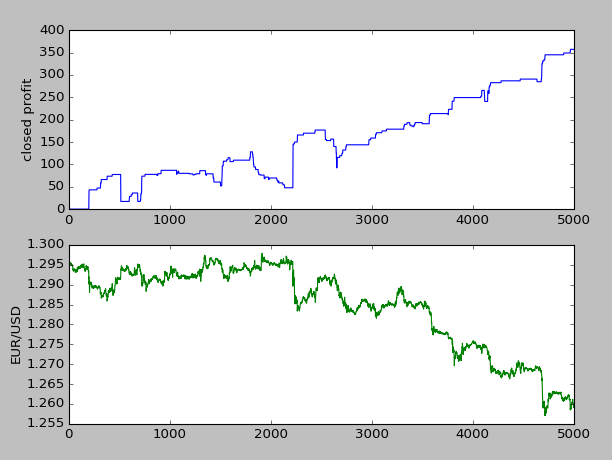
\includegraphics[scale = 0.5]{data-96-10000-20.png}
    \caption{This is a graph of the closed profit, on the control data.}
\end{figure}
\\
The next three result are where we keep the variables the same, but change the data we test on. So far we have had profit on each test, but with the large dataset, we get a closed profit of about -7250. Even though it might seem a lot, it is less than 3 dollars a day, spanning over 7 years. This shows that even with a confidence level on 96\%, you still might lose your money. By looking at the graph for the large data LINK TO GRAPH, we see that in the beginning, the classifier creates positive profit, but as we go on it looses. This might be because that we do not update the classifier each state.\\
\\
We therefore also made a test data, that was newer than both the large data and the control data. By looking at this graph LINK, we see that the classifier makes less trades, but also makes some larger mistakes. Even though we end in a profit with this data set, it is around 12 times less than in the control data. This confirms our theory that the classifier needs to be updated regularly to be able to work properly.
\\
\\
So far all our data have been collected over several day's, with a 5 min interval. We therefore decided to have a data set from a single day, with a 5 sec interval instead. This gave us the most profitable closed profit, at two times more than the control, a day.\\


\section{Conclusion}


Improvements:
A classifier that updates it self with newer data.
Using other features

\section{Terms \& abbrivations}
\begin{tabular}{l | l | l}
& Term or &\\
Domain & Abbreviation & Meaning\\
\hline
Trading & FX & Forex \\ 
Trading & Bid & An offer made by an investor,\\
& & a trader or a dealer to buy a security\\
Trading & Ask & The price a seller is willing to accept for a security\\
Trading & SMA & Simple Moving Average\\
Trading & MACD & Moving Average Convergence/Divergence\\
Trading & SAR & Parabolic SAR(Parabolic Stop and Reverse)\\
Machine Learning & NBC & Naive Bayes Classifiers\\
\end{tabular}


%plainnat
\bibliographystyle{plain}
\bibliography{roboFX}


\end{document}
